\documentclass[spanish,12pt, a4paper,twoside]{paper}

\let\oldsection\section
\def\section{\cleardoublepage\oldsection}

\usepackage{afterpage}


\newcommand\blankpage{%
    \null
    \thispagestyle{empty}%
    \addtocounter{page}{-1}%
    \newpage}

\usepackage[textwidth=15cm, textheight=22.5cm, top=3.5cm, bottom=3.5cm,left= 3cm,right=3cm]{geometry}


\usepackage[spanish]{babel}
%\usepackage[applemac]{inputenc} 
%POR DEFECTO SE ESTa USANDO EL PAQUETE PARA RECONOCER ACENTOS DE MAC, EN CASO DE USAR WINDOWS COMO SISTEMA OPERATIVO ELIMINAR LA LaNEA ANTERIOR E INTRODUCIR LA SIGUIENTE

\usepackage[utf8]{inputenc}

\usepackage{graphicx}
\usepackage{graphics}
\usepackage{amsmath,amssymb}
\usepackage{float}
\usepackage{changepage}
\usepackage{subcaption}


\usepackage{algorithm}
\usepackage{multirow}



\begin{document}
%\maketitle
%\thispagestyle{empty}
\begin{titlepage}

\newcommand{\HRule}{\rule{\linewidth}{0.5mm}} % Defines a new command for the horizontal lines, change thickness here

\renewcommand{\baselinestretch}{1.5}

\center % Center everything on the page
 
%	HEADING SECTIONS
%
\includegraphics[width=2.25cm]{recursos/logoFi.png}
  \hspace{9cm}

\includegraphics[width=3cm]{recursos/logo_urjc.jpg}
\\[1cm]

\textsc{\Large ESCUELA}\\[0.5cm]
\textsc{\large Universidad Rey Juan Carlos }
\\[3cm]


%	TITLE SECTION
 \HRule \\[0.4cm]
{ \huge \bfseries Titulo del Trabajo Fin de Máster}\\[0.4cm] % Title of your document
\HRule \\[2.5cm]

\textsc{\LARGE Trabajo Fin de Máster}\\[0.5cm] 
\textsc{\Large Máster Universitario En Formación del Profesorado de Ed.Secundaria, Bachillerato, FP e Idiomas }\\[2.5cm]

 %	AUTHOR SECTION
\begin{flushright}
\large
AUTOR: Abel de Andrés Gómez\\
TUTOR/ES: Nombre y Apellidos y \linebreak
                    Nombre y Apellidos
\end{flushright}

\vspace{1.3cm}

%	DATE SECTION
{ {2019}}\\[3cm]
%	LOGO SECTION

\vfill % Fill the rest of the page with whitespace

\end{titlepage}

\afterpage{\blankpage}
\pagenumbering{roman}


%	AGRADECIMIENTOS
\section*{AGRADECIMIENTOS}
Agrademos a...

%	RESUMEN
\section*{RESUMEN}
Extensión máxima de una página


%	SUMMARY
\section*{SUMMARY}
Extensión máxima de una página


%	ÍNDICE
\tableofcontents % indice de contenidos



%	INDICE DE FIGURAS Y TABLAS
\listoffigures
\listoftables



%	CAPaTULOS DEL TRABAJO FIN DE MaSTER
\newpage
\pagenumbering{arabic} 


\section{INTRODUCCIÓN}
\paragraph{}

En los últimos años, gracias al gran desarrollo tecnológico que se ha vivido tanto a nivel de computo (mejorando la eficiencia y el uso de los recursos disponibles) como a nivel de transmisión de datos (mejorando las comunicaciones), ha permitido a las organizaciones el almacenamiento de una gran cantidad de información.

\paragraph{}
Para comprender mejor este gran volumen de información, es necesario utilizar métodos, técnicas, herramientas además de personas con conocimientos (formando todas esta un vínculo estrecho) que permita y ayude a explotar, investigar, predecir y obtener información relevante para tomar decisiones de forma adecuada.
\paragraph{}
La organización educativa no ha quedado ajena a estas necesidades de una mejor comprensión de los datos. En este sentido, una unidad de Educación Secundaria Obligatoria de la Consejería de Educación de la Comunidad de Madrid ha planteado un problema.
\paragraph{}
El problema con el que se enfrentan cada día es la planificación de grupos para el siguiente curso. Esta planificación es la base para poder decidir donde se escolariza cada alumno y como se va a repartir la plantilla del profesorado según sus especialidades. Conocer el número de grupos permite, por tanto, un óptimo reparto de la plantilla de docentes y de recursos. De esta forma, además, se evita la existencia de grupos sobrepoblados.

\paragraph{}
Desde esta unidad, han informado sobre aspectos sobre los que trabajan para poder realizar una predicción acerca del número de grupos para curso venidero. 

\paragraph{}
Estos aspectos son:

\begin{enumerate}
\item Escolaridad del curso actual.
\begin{itemize}
\item Número de alumnos y grupos de un determinado centro.
\item El número de alumnos por aula (también conocido como ratio).
\item Matriculación de nuevos alumnos.
\begin{itemize}
\item Principalmente alumnos que superan el nivel de 6º de primaria y pasan a 1º de ESO.
\end{itemize}
\end{itemize}

\item Bilingüismo del centro. Muchos alumnos optan por centros bilingües para su mejor formación, por lo que estos centros suelen tener más demanda de alumnos.
\item Posibilidad de creación de nuevas zonas urbanas cerca del centro. 
\item Posibilidad de apertura o cierre de centros educativos. El cierre de por ejemplo, de un centro privado, provocara una mayor tasa de matriculación de los centros contiguos. 
\item Porcentaje de aprobados. Los alumnos que están ya matriculados tienen prioridad sobre los nuevos alumnos, por lo tanto, si existe una alta tasa de suspensos, quedan pocas plazas de admisión de nueva matricula.
\item El número y la aparición de nuevas enseñanzas. La oferta de nuevas enseñanzas atraerá a nuevos alumnos al centro, incrementando así el número de matriculaciones.
\end{enumerate}

\paragraph{}
La unidad actualmente utiliza herramientas manuales para conseguir conocer el número de grupos, indicando que es un trabajo mecánico y con herramientas obsoletas, evitando la posibilidad de inclusión de nuevas variables o factores que impliquen nuevos resultados.
\paragraph{}
Propone dar una solución al problema actual mediante el uso de herramientas y métodos que automaticen dichas tareas y proponga, además, nuevas variables o factores que puedan influir en la toma de decisión. 

\section{JUSTIFICACIÓN TEÓRICA}
%https://www.thetechedvocate.org/8-ways-machine-learning-will-improve-education/
En primer lugar, y, antes de comenzar la investigación, se ha acudido a los datos del INE (Instituto Nacional de Estadística) y a los del ministerio de educación, ciencia y deportes (MECD).
Como la investigación va dirigida a los alumnos de la ESO, se ha buscado información respectiva a este nivel educativo. 


\section{PROPUESTA DE INTERVENCIÓN}
\paragraph{}
Con el objetivo de resolver el problema comentado en los apartados anteriores, se plantea el uso de la ciencia de datos como proceso para descubrir relaciones entre los datos, que sean significativas. Además, se van a buscar patrones y tendencias en los datos que ayuden a la toma de decisiones.
\paragraph{}
En primer lugar, se debe tener en cuenta que la ciencia de datos aúna métodos y tecnologías que provienen del campo de las matemáticas, la estadística y la informática entre las que se pueden encontrar el análisis descriptivo o exploratorio, el aprendizaje automático (“machine learning”), el aprendizaje profundo (“Deep learning”), etc. \cite{Marin2018}. En esta propuesta de intervención, se va a centrar en el análisis descriptivo y el aprendizaje automático.
\paragraph{}
El análisis descriptivo, como ya se ha comentado, va a ser útil para observar características de los propios datos. Entre estas características se va a poder observar cuales son las variables que más convienen al estudio por su importancia, utilizando técnicas como el análisis principal de componentes. Se puede observar también la correlacion entre las variables, sobretodo.
\paragraph{}
El aprendizaje automático, se divide en dos áreas: el aprendizaje supervisado y el no supervisado. 

\begin{itemize}
\item El aprendizaje supervisado se basa en algoritmos que intentan encontrar una función, que, dadas las entradas, asigne unas salidas adecuadas. Estos algoritmos se entrenan mediante datos históricos y de esta forma aprende a asignar salidas adecuadas en función de dichas entradas, dicho de otra forma, predice el valor de salida. A su vez, el aprendizaje supervisado se divide en regresión (si la salida es de tipo numérico) y clasificación (si la salida es del tipo categórico). \cite{Recuero2017}
\item El aprendizaje no supervisado se utiliza en datos en los que existen variables de entrada, pero no existen variables de salida para dichas variables de entrada. Por consiguiente, solo se puede describir la estructura de los datos, para intentar conseguir algún tipo de estructura u organización que simplifique el análisis.\cite{Recuero2017}
\end{itemize}


\section{DISEÑO DE INVESTIGACIÓN}
En este apartado, se va a presentar la forma en la que se va a realizar la investigación. En primer lugar, se va a realizar un proceso ETL, posteriormente se va a realizar un análisis descriptivo mediante sus técnicas que se explicaran posteriormente, además se va a incluir técnicas de aprendizaje no supervisada en este análisis.
Una vez que se ha realizado el análisis descriptivo, se va a realizar un análisis predictivo. En este análisis se va a utilizar técnicas de aprendizaje supervisadas.

\subsection{Proceso de Extracción, Extracción y Carga}
En primer lugar, se va a realizar un tratamiento de datos, para ello, se utilizará la técnica conocida como ETL (extracción, transformación y carga) que consiste básicamente en obtener los datos de la fuente de origen (bases de datos, ficheros Excel, ficheros JSON, etc), seleccionar aquellos datos que convengan al estudio, transfórmalos según las necesidades que se tenga y depurarlos (evitando así datos erróneos). (Prakash, 2017) (Guillermo Matos, 2006) (Sharma, 2014).
Para realizar este tratamiento, se ha va a utilizar Pentaho BI, que es un conjunto de programas libres para realizar entre otras muchas actividades, las técnicas de ETL. Concretamente, se ha utilizado la herramienta Spoon para desarrollar esta técnica. 
Una vez que se tienen los datos limpios y estructurados, se pueden realizar dos operaciones:

\begin{enumerate}
\item  En primer lugar, se pueden almacenar dichos datos en una base de datos y seguir utilizando Pentaho BI para poder crear cuadros de mandos e informes. 
\item  En segundo lugar, se puede almacenar la información en un texto plano para poder trabajar con herramientas de análisis descriptivo y predictivo. Estos análisis se van a realizar a través del entorno y lenguaje de programación R, que es una referencia en el ámbito de la estadística.
\end{enumerate}

\subsection{Análisis Descriptivo}
El análisis predictivo (también conocido como estadísticas predictivas) se encarga de resumir los datos en bruto para que puedan ser interpretados. Estos análisis son útiles ya que permiten aprender sobre comportamientos o patrones pasados e entender cómo pueden influir en los resultados futuros. En este tipo de análisis se van a utilizar tanto métodos graficos como medidas resumen.

En primer lugar, se debe estudiar el tipo de datos de cada variable a estudiar, se debe clasificar las variables según sean categóricas (dicotómicas o polinómicas) o numéricas (discretos o continuos). El tipo de datos permite decidir qué tipo de análisis estadístico utilizar.
Una vez que se tienen claro el tipo de datos utilizados, se van a utilizar los principales estadísticos como la media, la mediana, las desviaciones típicas, etc.
Posteriormente se va a utilizar la matriz de varianzas y covarianzas, que indicaran la variabilidad de los datos y la información sobre las posibles relaciones lineales entre las variables. 

Por otro lado, se va a estudiar la correlación de las variables mediante la matriz de correlación. Esta matriz contendrá los coeficientes de correlación.\cite{JMMarin}. La matriz de correlación, se utilizará fundamentalmente por pares entre las variables y la variable a predecir.

También se va a estudiar la matriz de correlaciones parciales, que estudia la correlación entre pares de variables eliminando el efecto de las restantes.\cite{JMMarin}

Los datos categóricos se van a representar en tablas de frecuencias, gráficos de barras y gráficos de sectores. Los datos numéricos se van a representar mediante histogramas, boxplot y diagramas QQ-Plot o Grafico Cuantil-Cuantil. \cite{Orellana2001}

Mediante el boxplot se puede observar aspectos como la posición, dispersión, asimetría, longitud de colas y los datos anómalos (outliers). 
El QQ-plot se va a utilizar para evaluar la cercanía de los datos a una distribución. \cite{Orellana2001}

%(https://www.sergas.es/gal/documentacionTecnica/docs/SaudePublica/Apli/Epidat4/Ayuda/Ayuda_Epidat_4_Analisis_descriptivo_Octubre2014.pdf)
Por otro lado, se va a complementar el análisis descriptivo mediante el aprendizaje no supervisado, donde también se extraerán otras características de los datos.


\subsubsection{Aprendizaje No Supervisado}
\begin{enumerate}
\item Algoritmos de Clustering
\item Análisis de Componentes Principales
\item Descomposición en valores singulares
\item Analisis de componentes independientes
\item Stepwise Regression
\end{enumerate}

%https://www.fisterra.com/mbe/investiga/10descriptiva/10descriptiva.asp#top
%http://www.uco.es/zootecniaygestion/img/pictorex/27_12_49_7.pdf
%https://machinelearningmastery.com/descriptive-statistics-examples-with-r/
%http://cms.dm.uba.ar/academico/materias/verano2015/estadisticaQ/descriptiva.pdf

\subsection{Análisis Predictivo}
\paragraph{}
Una vez terminado el análisis descriptivo, se va a realizar un análisis predictivo. Se debe tener en cuenta, que, dentro de la ciencia de datos, existen técnicas de aprendizaje automáticas, cuyo objetivo es la construcción de un sistema que sea capaz de aprender a resolver problemas sin la intervención de un humano. \cite{Marin2018}.
\paragraph{}
El aprendizaje supervisado consiste en la búsqueda de patrones en datos históricos relacionando todas las variables con una especial (conocida como variable objetivo). Los algoritmos que se utilizan en el aprendizaje supervisado se encarga de buscar patrones en los datos. A este proceso se conoce como entrenamiento de los datos. Una vez que se tienen los patrones, se aplican a los datos de prueba. Los datos de entrenamiento suelen ser una selección aleatoria y única de los datos históricos de un 70\% del total. Los datos de prueba son el restante 30\%. \cite{Manguart2017}
Algunos de los algoritmos que se van a utilizar son:
\begin{enumerate}
\item Arboles de decisión
\paragraph{} Se basa en el descubrimiento de patrones a partir de ejemplos. Un árbol de decisión está formado por un conjunto de nodos (de decisión) y de hojas (nodos-respuesta).
\paragraph{} 
Los nodos están asociados a los atributos y tiene varias ramas que salen de él (dependiendo de los valores que tomen la variable asociada). Estos nodos pueden asemejarse a preguntas que, dependiendo de la respuesta que conlleve, se tomara un flujo en las ramas salientes.
\paragraph{} 
Los nodos respuesta están asociados a la clasificación que se desea proporcionar, devolviendo así la decisión del árbol con respecto al ejemplo de entrada utilizado.

\begin{figure*}[htb]
\centering
 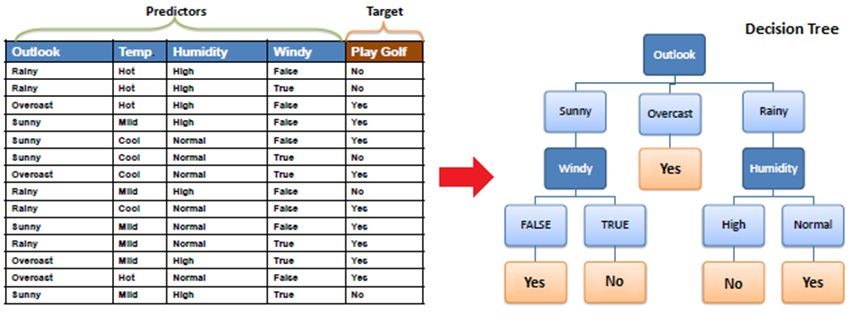
\includegraphics[width=0.8\textwidth]{recursos/arbol_decision_img1}
\caption{Funcionamiento Arboles Decisión}
\label{fig:fun_arb_dec}
\end{figure*}


\item Análisis de Componentes Principales
\paragraph{} prueba
\item Descomposición en valores singulares
\item Analisis de componentes independientes
\item Stepwise Regression
\end{enumerate}

\subsubsection{Aprendizaje No Supervisado}
\begin{enumerate}
\item Algoritmos de Clustering
\item Análisis de Componentes Principales
\item Descomposición en valores singulares
\item Analisis de componentes independientes
\item Stepwise Regression
\end{enumerate}


\section{ANÁLISIS DE RESULTADOS}

\section{CONCLUSIONES}

\section{SOBRE LAS REFERENCIAS}

La bibliografaa o referencias deben aparecer siempre al final de la tesis, incluso en aquellos casos donde se hayan utilizado notas finales. La bibliografaa debe incluir los materiales utilizados, incluida la edician, para que la cita pueda ser facilmente verificada. 

\bigskip
{\bf Citar dentro del texto:}

Las fuentes consultadas se describen brevemente dentro del texto y estas citas cortas se amplaan en una lista de referencias final, en la que se ofrece la informacian bibliografica completa. 

La cita dentro del texto es una referencia corta que permite identificar la publicacian de dande se ha extraado una frase o parafraseado una idea, e indica la localizacian precisa dentro de la publicacian fuente. Esta cita informa del apellido del autor, la fecha de publicacian y la pagina (o paginas) y se redacta de la forma que puede verse a travas de los siguientes ejemplos:

Cuando se citan las palabras exactas del autor deben presentarse entre comillas e indicarse, tras el apellido del autor y, entre parantesis, la fecha de publicacian de la obra citada, seguida de la/s pagina/s.

Si lo que se reproduce es la idea de un autor (no sus palabras exactas) no se pondran comillas y se indicara, entre parantesis, el apellido del autor seguido de la fecha de publicacian de la obra a la que se refiere.

No se puede eliminar una parte del texto citado sin seaalarse; debe indicarse siempre con puntos suspensivos entre corchetes [...]

Ejemplos de como citar una referencia en el texto son los siguientes \cite{Ashtiani2014} o \cite{Ashtiani2014,Mateos2009,Vicente2016}.


\bigskip
{\bf Camo ordenar las referencias:}
\begin{enumerate}
\item Las referencias bibliograficas deben presentarse ordenadas alfabaticamente por el apellido del autor, o del primer autor en caso de que sean varios.
\item Si un autor tiene varias obras se ordenaran por orden de aparician.
\item Si de un mismo autor existen varias referencias de un mismo aao se especificaran los aaos seguidos de una letra minascula y se ordenaran alfabaticamente.
\item Si son trabajos de un autor en colaboracian con otros autores, el orden vendra indicado por el apellido del segundo autor, independientemente del aao de publicacian. Las publicaciones individuales se colocan antes de las obras en colaboracian.
\end{enumerate}

\bigskip
{\bf Camo citar un artaculo de revista}

Un artaculo de revista, siguiendo las normas de la APA, se cita de acuerdo con el siguiente esquema general:
Apellido(s), Iniciales del nombre o nombres. (Aao de publicacian). Tatulo del artaculo. Tatulo de la revista en cursiva, volumen de la revista (namero del fascaculo entre parantesis), primera pagina- altima pagina del artaculo.

\bigskip
{\bf Camo citar una monografaa/libro}

Las monografaas, siguiendo las normas de la APA, se citan de acuerdo con el siguiente esquema general:
Apellido(s), Iniciales del nombre. (Aao de publicacian). Tatulo del libro en cursiva. Lugar de publicacian: Editorial.
Opcionalmente podremos poner la mencian de edician, que ira entre parantesis a continuacian del tatulo; y, si fuera el caso el volumen que ira en cursiva.

\bigskip
{\bf Camo citar un capatulo de un libro}

Los capatulos de los libros se citan de acuerdo con el siguiente esquema general:
Apellido(s), Iniciales del nombre o nombres. (Aao). Tatulo del capatulo. En A. A. Apellido(s) Editor A, B. B. Apellido(s) Editor B, y C. Apellido(s) Editor C (Eds. o Comps. etc.), Tatulo del libro en cursiva (pp. xxx-xxx). Lugar de publicacian: Editorial.

\bigskip
{\bf Camo citar un acta de un congreso}

Apellido(s), Iniciales del nombre o nombres. (Aao). Tatulo del trabajo. En A. A. Apellido(s) Editor A, B. B. Apellido(s) Editor B, y C. Apellido(s) Editor C (Eds. o Comps. etc.), Nombre de los proceedings en cursiva (pp. xxx-xxx). Lugar de publicacian: Editorial.

\bigskip
{\bf Camo citar tesis doctorales, trabajos fin de master o proyectos fin de carrera}

Apellido(s), Nombre. (Aao). Tatulo de la obra en cursiva. (Tesis doctoral). Institucian a acadamica en la que se presenta. Lugar.

\bigskip
{\bf Camo citar un recurso de Internet}

Los recursos disponibles en Internet pueden presentar una tipologaa muy variada: revistas, monografaas, portales, bases de datos... Por ello, es muy difacil dar una pauta general que sirva para cualquier tipo de recurso.
Como manimo una referencia de Internet debe tener los siguientes datos:
\begin{enumerate}
\item Tatulo y autores del documento.
\item Fecha en que se consulta el documento.
\item Direccian (URL auniform resource locatora)
\end{enumerate}

Veamos, a travas de distintos ejemplos, camo se citan especaficamente algunos tipos de recursos electranicos.

Monografaas:
Se emplea la misma forma de cita que para las monografaas en versian impresa. Debe agregar la URL y la fecha en que se consulta el documento

Artaculos de revistas:
Se emplea la misma forma de cita que para los artaculos de revista en versian impresa. Debe agregar la URL y la fecha en que se consulta el documento.

Artaculos de revistas electranicas que se encuentran en una base de datos:
Se emplea la misma forma de cita que para los artaculos de revista en versian impresa, pero debe aaadirse el nombre de la base datos, la fecha en que se consulta el documento.

\section*{ANEXOS}


\section*{BIBLIOGRAFÍA}

%	REFERENCIAS
\newpage

\begin{thebibliography}{00}
%\bibitem{Ashtiani2014}  Ashtiani, M.H.Z., Ahmadabadi, M.N., Araabi, B.N. (2014). Bandit-based local feature subset selection. \emph{Neurocomputing} 138, 371--382.
%\bibitem{Berry1985} Berry, D., Fristedt, B. (1985). \emph{Bandit problems}. London: Chapman and Hall.
%\bibitem{Figueira2005} Figueira, J., Mousseau, V., Roy, B. (2005). Electre methods. En J. Figueira, S. Greco y M. Erghott (Eds.), \emph{Multiple criteria decision analysis. State of the art survey} (pp. 133--162). New York: Springer.
%\bibitem{Li2010} Li, L., Chu, W., Langford, J., Schapire, R.E. (2010). A contextual-bandit approach to personalized news article recommendation. En \emph{Proceedings of the 19th International Conference on World Wide Web} (pp. 661--670). New York: ACM.
%\bibitem{Mateos2009} Mateos, A., Jimanez, A. (2009). A trapezoidal fuzzy numbers-based approach for aggregating group preferences and ranking decision alternatives in MCDM. En M. Erghott, C.M. Fonseca, X. Gandibleux, H. Jao y M. Servaux (Eds.). \emph{Evolutionary multi-criterion optimization} (pp. 365--379). Berlin: Springer.
%\bibitem{Sutton1998} Sutton, R. Barto, A. (1998). \emph{Reinforcement learning, an introduction}. Cambridge: MIT Press.
%\bibitem{Thompson1933} Thompson, W.R. (1933). On the likelihood that one unknown probability exceeds another in view of the evidence of two samples. \emph{Biometrika} 25(3-4), 285--294.
%\bibitem{Vicente2016} Vicente, E. (2016). \emph{Analisis y gestian del riesgo en los sistemas de informacian: Un enfoque borroso}. (Tesis doctoral). Universidad Politacnica de Madrid, Madrid.
\bibitem{Manguart2017}Manguart, A. (2017, 13 junio). Conceptos básicos del aprendizaje supervisado (para personas no técnicas) [Publicación en un blog]. Recuperado 15 enero, 2019, de https://medium.com/@manguart/machine-learning-conceptos-básicos-del-aprendizaje-supervisado-para-personas-no-técnicas-142bbb222140
\bibitem{Marin2018} Marín, J. L. (2018, 5 abril). \emph{Ciencia de datos, machine learning y deep learning} (Comunicado de prensa). Recuperado 17 enero, 2019, de https://datos.gob.es/es/noticia/ciencia-de-datos-machine-learning-y-deep-learning
\bibitem{JMMarin}Marín, J. M. (s.f.). Estadística Descriptiva Univariante [Tema Universitario]. Recuperado 17 enero, 2019, de http://halweb.uc3m.es/esp/Personal/personas/jmmarin/esp/AMult/tema2am.pdf
\bibitem{Orellana2001}Orellana, L. (2001). Introducción. In L. Orellana (Ed.), Estadística Descriptiva (pp. 1–64). Recuperado de http://www.dm.uba.ar/materias/estadistica\_Q/2011/1/modulo\%20descriptiva.pdf
\bibitem{Recuero2017}Recuero, P. (2017, 16 noviembre). Los 2 tipos de aprendizaje en Machine Learning: supervisado y no supervisado [Publicación en un blog]. Recuperado 17 enero, 2019, de https://data-speaks.luca-d3.com/2017/11/que-algoritmo-elegir-en-ml-aprendizaje.html

\end{thebibliography}
\end{document}

